\documentclass[preprint]{sigplanconf}

\usepackage{graphicx}
\usepackage{longtable}
\usepackage{comment}
\usepackage{amsmath}
\usepackage{mdwlist}
\usepackage{txfonts}
\usepackage{xspace}
\usepackage{amstext}
\usepackage{amssymb}
\usepackage{stmaryrd}
\usepackage{proof}
\usepackage{multicol}
\usepackage[nodayofweek]{datetime}
\usepackage{etex}
\usepackage[all, cmtip]{xy}
\usepackage{xcolor}
\usepackage{listings}
\usepackage{multicol}
\usepackage{bm}


\newtheorem{theorem}{Theorem}[section]
\newtheorem{lemma}[theorem]{Lemma}
\newtheorem{proposition}[theorem]{Proposition}
\newtheorem{corollary}[theorem]{Corollary}

\newcommand{\xcomment}[2]{\textbf{#1:~\textsl{#2}}}
\newcommand{\amr}[1]{\xcomment{Amr}{#1}}
\newcommand{\roshan}[1]{\xcomment{Roshan}{#1}}

\newcommand{\ie}{\textit{i.e.}\xspace}
\newcommand{\eg}{\textit{e.g.}\xspace}

\newcommand{\lcal}{\ensuremath{\lambda}-calculus}
\newcommand{\G}{\ensuremath{\mathcal{G}}\xspace}

\newcommand{\code}[1]{\lstinline[basicstyle=\small]{#1}\xspace}
\newcommand{\name}[1]{\code{#1}}

\def\newblock{}

\newenvironment{floatrule}
    {\hrule width \hsize height .33pt \vspace{.5pc}}
    {\par\addvspace{.5pc}}

%subcode-inline{bnf-inline} name langRev
%! swap+ = \mathit{swap}^+
%! swap* = \mathit{swap}^*
%! dagger =  ^{\dagger}
%! assocl+ = \mathit{assocl}^+
%! assocr+ = \mathit{assocr}^+
%! assocl* = \mathit{assocl}^*
%! assocr* = \mathit{assocr}^*
%! identr* = \mathit{uniti}
%! identl* = \mathit{unite}
%! dist = \mathit{distrib}
%! factor = \mathit{factor}
%! (o) = \fatsemi
%! (;) = \fatsemi
%! (*) = \times
%! (+) = +

%subcode-inline{bnf-inline} regex \{\{(((\}[^\}])|[^\}])*)\}\} name main include langRev
%! Gx = \Gamma^{\times}
%! G = \Gamma
%! [] = \Box
%! |-->* = \mapsto^{*}
%! |-->> = \mapsto_{\ggg}
%! |--> = \mapsto
%! |- = \vdash
%! ==> = \Longrightarrow
%! <== = \Longleftarrow
%! <=> = \Longleftrightarrow
%! <-> = \leftrightarrow
%! ~> = \leadsto
%! -o = \multimap
%! ::= = &::=&
%! /= = \neq
%! forall = \forall
%! exists = \exists
%! empty = \epsilon
%! langRev = \Pi
%! langRevT = \Pi^{o}
%! langRevEE = \Pi^{\eta\epsilon}
%! theseus = Theseus
%! * = \times

%%%%%%%%%%%%%%%%%%%%%%%%%%%%%%%%%%%%%%%%%%%%%%%%%%%%%%%%%%%%%%%%%%%%%%%%%%%%%%%%

\begin{document}

\conferenceinfo{ICFP'12}{}
\CopyrightYear{}
\copyrightdata{}
\titlebanner{}
\preprintfooter{}

\title{Functional Pearl: \\ Programming with Negative and Fractional Types} 
\authorinfo{Roshan P. James}
           {Indiana University}
           {rpjames@indiana.edu}
\authorinfo{Amr Sabry}
           {Indiana University}
           {sabry@indiana.edu}
\maketitle

\begin{abstract}
  Every functional programmer knows about sum and product types, $a+b$ and
  $a*b$ respectively. Negative and fractional types, $a-b$ and $a/b$
  respectively, are much less known and their computational interpretation is
  unfamiliar and often complicated. We show that in a programming model in
  which information is preserved (such as the model introduced in our recent
  paper on \emph{Information Effects}), negative and fractional types have
  particularly intuitive and natural computational
  interpretations. Intuitively, values of negative types are values that flow
  ``backwards'' to satisfy demands, and values of fractional types are values
  that represent first-class pattern clauses. The combination of negative and
  fractional types allow a programmer to express a wide range of programming
  idioms, including higher-order functions, delimited continuations,
  speculative computation, logic programming, and more. 
\end{abstract}

%%%%%%%%%%%%%%%%%%%%%%%%%%%%%%%%%%%%%%%%%%%%%%%%%%%%%%%%%%%%%%%%%%%%%%%%%%%%%%%%
\category{D.3.1}{Formal Definitions and Theory}{}
\category{F.3.2}{Semantics of Programming Languages}{}
\category{F.3.3}{Studies of Program Constructs}{Type structure}

\terms
Languages, Theory

\keywords Arrows, Linear logic, Quantum computing, Reversible logic.

%%%%%%%%%%%%%%%%%%%%%%%%%%%%%%%%%%%%%%%%%%%%%%%%%%%%%%%%%%%%%%%%%%%%%%%%%%%%%%%%
\section{Introduction}

We show a deep symmetry between functions and delimited continuations,
values and continuations that arises in {{langRev}} in a manner that
is reminiscent of Filinksi's Symmetric \lcal
~\cite{Filinski:1989:DCI:648332.755574}. The symmetry arises by
extending {{langRev}} with a notion of additive duality over the
monoid {{(+, 0)}} by including {{eta}} and {{eps}} operators of
Compact Closed Categories. The resulting dual types, which we denote
{{-b}}, have a time traveling ``backward information flow''
interpretation and allow for the encoding of higher-order function and
iteration via the construction of {{trace}} operators, thereby making
the extended language {{langRevEE}} a Turing-complete reversible
programming language with higher-order functions and first-class
delimited continuations.

We introduced this thesis that computation should be based on isomorphisms
that preserve information~\cite{infeffects}. Since Filinski, we've had the
idea that values and continuations are like mirror images. In a conventional
language, the negative (continuation) side is implicit and we introduce
information effects on the positive. Trying to recover the duality from this
distorted positive side has always been messy. Now it looks clean because we
have kept the positive side pure.

The way to think about something of type $A$ is that it is a value we have
produced. The way to think about something of type $-A$ is that is a value we
have already consumed. 

Other interpretations of the types of think about. The first one is
arithmetic obviously. Another one is languages consisting of sets of
string. The type 0 is the empty set, the type 1 is the set containing the
empty word, the $+$ constructor corresponds to union, and the $*$ constructor
corresponds to concatenation. The constructor $-$ would not correspond to set
difference however. It would correspond to marking the elements in the set as
``consumed'' so that if we take the union and a ``consumed'' element appears
in the other set, the two cancel. This makes it clear that concatenating a
produced $a$ and a consumed $b$ is not the same as concatenating a consumed
$a$ and a produced $b$. They really need to be kept separate. Incidentally,
division would be defined as follows:
\[
L_1 / L_2 = \{ x ~|~ xy \in L_1 \mbox{~for~some~} y \in L_2 \}
\]

%%%%%%%%%%%%%%%%%%%%%%%%%%%%%%%%%%%%%%%%%%%%%%%%%%%%%%%%%%%%%%%%%%%%%%%%%%%%%%%%
\section{Value Producers and Consumers}

Consider the following ways of purchasing an item that costs \$20.00:

\begin{enumerate}
\item You produce a \$20.00 bill and give it to the seller.
\item You use a credit card. 
\end{enumerate}
In both cases the seller receives the money immediately but there is a subtle
difference. In the second transaction, nobody has yet produced the money that
the seller has received: instead a \emph{debt} is generated and this debt
travels ``backwards'' towards the bank and (hopefully) reconciled there.

Computationally we model the first transaction using essentially the identity
function which receives a \$20.00 bill as input from the buyer and propagates
it on its output to the seller. The second transaction is more
complicated. We model it as shown in the circuit below:

FIGURE

There are two ways to understand this circuit that are both quite
instructive. Let's first examine the type structure of each of the
combinators that comprise the circuit. The first combinator on the right
outputs \$20.00 to the seller. This \$20.00 is produced from nothing so to
speak by generating an equivalent debt that travels backwards. COMPLETE BASED
ON THE FIGURE.

The other way is to follow the execution. It goes forward in time so to speak,
comes back, and then goes forwards again.

\paragraph*{Continuations.} The idea of using negative types to model
information flowing backwards, demand for values, continuations, etc. goes
back to at Filinski's thesis. We recall these connections below but we first
note that all these systems are complicated because in all these systems
information can be ignored, destroyed, or duplicated. Clearly the possibility
of erasure of information would mean that our credit card transaction is
incorrect. In our work, information is maintained and hence we have a
guarantee that, in a closed program, the debt must be accounted and paid for.

\paragraph*{Filinski~\cite{Filinski:1989:DCI:648332.755574}.}
In his Masters thesis, Filinski proposes that continuations are a
\emph{declarative} concept. He, furthermore, introduces a symmetric extension
of the $\lambda$-calculus in which values and continuations are treated as
opposites. This is essentially what we are proposing with one fundamental
difference: our underlying language is not the $\lambda$-calculus but a
language of pure isomorphisms in which information is preserved. This shift
of perspective enables us to distill and generalize the duality of values and
continuations: in particular, in the conventional $\lambda$-calculus setting
values and continuations can be erased and duplicated which makes it
difficult to maintain the correspondence between a value and its negative
counterpart. In contrast, in our setting, one can start from the empty type
$0$, introduce a positive value and its negative counterpart, and let each of
these flow in arbitrary ways. The entire framework guarantees that neither
the value nor its negative counterpart will be deleted or duplicated and
hence that, in any closed program, the ``debt'' corresponding to the negative
value is paid off exactly once. 

The forward and backward executions in our framework correspond to
call-by-value and call-by-name. This duality was observed by Filinski and
others following him but it is particularly clean in our framework.

\paragraph*{Subtraction} Wadler the reloaded paper, does not consider the
subtraction type because its ``computational interpretation is not
familiar.'' Curien and Herbelin study duality in classical logic, show that
it exchanges call-by-value and call-by-name. They extend classical natural
deduction with subtraction but give it no computational meaning. Crolard (in
the formulae-as-types interpretation of subtractive logic) address the
computational interpretation of substraction. He explains the type $A-B$ as
the of \emph{coroutines} with a local environment of type $A$ and a
continuation of type $B$. The description is complicated by what is
essentially the desire to enforce linearity constraints so that coroutines
cannot access the local environment of other coroutines. Must cite Selinger
control categories in this context of duality but I am not sure what to say:
it assumes cartesian closed categories for one thing and not symmetric
monoidal ones. Ariola, Herbelin, and Sabry also use subtractive types to
explain delimited continuations. 

\paragraph*{Linear Logic} In accounts that are linear, the value and
continuation that comprise the substractive type need to be constrained to
``stay together.'' This can be achieved by various restrictions. In this work
we have no such constraints, the negative value can flow anywhere. The entire
system guarantees that any closed program would have to account for it. We
don't have to introduce special constraints to achieve that. Zeilberger in
the paper on polarity and the logic of delimited continuations uses polarized
logic: he shows that if positive and negative values are completely symmetric
except that answer types are positive, then the framework accommodates
delimited continuations. But he interprets negative values are control
operators, or as values defined by the shape of their continuations. We
simply interpret values of negative type as values flowing in the ``other''
direction.

\paragraph*{Int Construction.}
For a traced monoidal category {{C}} the Int construction produces a
Compact Closed Category called Int {{C}} \cite{joyal1996traced}.
Further we know that the target of the Int construction is isomorphic
to the target of \G construction of Abramsky \cite{Abramsky96:0} from
Haghverdi. However, note that the {{langRevEE}} is not the same as the
image of the Int construction on {{langRevT}}, since the the later
lacks a multiplicative tensor that distrbutes over the additive tensor
in Int {{langRevT}}.

\paragraph*{Recursion.} In our previous work we introduce recursive types and
trace operators. This is dangerous here because infinite loops allow us to
prolong paying the debt for as long as we want.


\paragraph*{GoI machines} 
We can now encode the GoI machine of Mackie \cite{Mackie2011,DBLP:conf/popl/Mackie95}.


%%%%%%%%%%%%%%%%%%%%%%%%%%%%%%%%%%%%%%%%%%%%%%%%%%%%%%%%%%%%%%%%%%%%%%%%%%%%%%%%
\section{Additive Duality in {{langRev}} }

%%%%%%%%%%%%%%%
\subsection{Syntax}

%subcode{bnf} include main
% Values, v = () | (v, v) | L v | R v
% Combinators, c &=& iso | c (;) c | c(+)c | c (*) c 
%
% Sequential Contexts, P, F = [] | P:c
% Parallel Contexts, D = [] 
%                     &|& D:(P| [](+)c| F)
%                     &|& D:(P| c(+)[]| F)
%                     &|& D:(P| [] (*) c v| F)
%                     &|& D:(P| [] (*) v c| F)
%                     &|& D:(P| c v (*)  []| F)
%                     &|& D:(P| v c (*) []| F)
%
%
% Machine States  = D[P| c v| F] | D[P| v c| F]
% Start State  = [][[]| v c| []]
% Stop State  = [][P| c v| []]

Combinator reconstruction, {{P[c]}}:
%subcode{opsem} include main
% [](c) '= c
% P:c'(c) '= P(c'(;)c)

%%%%%%%%%%%%%%%%%%%%%
\subsection{Operational Semantics}

The small step semantics present for {{langRev}} below work
symmetrically for forward and backward evaluation.

\begin{itemize}
\item 
Basic reduction of an isomorphism. Note that the evaluation leaves the
adjoint of the combinator behind. This will become important when we
reverse the direction of computation.
%% %subcode{opsem} include main
%% % <P; F; iso v; D>      &|-->& <P; F; v'~ iso{dagger}; D>

%subcode{opsem} include main
% D[P|v iso| F]      &|-->& D[P| iso{dagger} v| F]

\item
Sequencing involves pushing and popping from the Future and Past
continuations:
%subcode{opsem} include main
% D[P|v (c1(;)c2)| F]  &|-->& D[P| v c1| F:c2]
% D[P| c1 v| F:c2] &|-->& D[P:c1| v c2| F]


\item
Parallel composition, captures the current Future and Past and extends
the parallel context.
%subcode{opsem} include main
% D[P|(L v) c1 (+) c2| F] &|-->& D:(P|[](+)c2|F)[ []| v c1| [] ]
% D[P| (R v) c1 (+) c2| F] &|-->& D:(P|c1(+)[]|F)[ []| v c2| [] ]
% D:(P|[](+)c2|F)[P'|c1 v| [] ]  &|-->& D[P|(P'(c1)(+)c2{dagger}) (L v)| F] 
% D:(P|c1(+)[]|F)[P'| c2 v| [] ] &|-->& D[P|(c1{dagger}(+)P'(c2)) (R v)| F]


\item
Similarly for products:
%subcode{opsem} include main
% D[P| (v1, v2) c1 (*) c2| F] &|-->& D:(P| [] (*) v2 c2|F)[ []| v1 c1| [] ]
% D:(P|[] (*) v2 c2|F)[P'| c1 v1| [] ] &|-->& D:(P|P'(c1) v1 (*) []|F)[ []| v2 c2| [] ]
% D:(P|c1 v1(*) []|F)[P'|c2 v2| [] ]  &|-->& D[P|c1(*)P'(c2) (v1, v2)| F]


and symmetrical rules for evaluation along the second branch. 
%subcode{opsem} include main
% D:(P|v1 c1 (*) []|F)[P'| c2 v2| [] ] &|-->& D:(P,[] (*) P'(c2) v2,F)[ []| v1 c1| [] ]
% D:(P|[] (*) c2 v2|F)[P'|c1 v1| [] ] &|-->& D[P |P'(c1) (*) c2 (v1, v2)| F]

The later two rules will be relevant only for reverse execution. 

\end{itemize}


%%%%%%%%%%%%%%%%%
\section{Rules for {{eta}} and {{eps}} }

The operation {{eps}} reverses the direction of a particle by
reversing the world. 

Note that we deviate from the categorical definition of {{eta}} and
{{eps}} slightly in that they swap the order of {{-b}} and {{b}} in
choice of {{eta}}. This however does not affect us, because we deal
with a symmetric category.

\begin{itemize}
\item Grammar
%subcode{bnf} include main
% Values, v = () | (v, v) | L v | R v | -v
% Isomorphisms, iso &=& ... | eta | eps
% Combinators, c &=& iso | c (;) c | c(+)c | c (*) c 

\item
Type judgement.
%subcode{opsem} include main
% eta &: 0 <-> (-b) + b :& eps

%subcode{proof} include main
%@ |- v : b
%@@ |- -v : -b

\item
Operational Semantics.
%subcode{opsem} include main
% D[P| (R v) eps| F]      &|-->&  D{dagger}[F | eps (L (-v))| P]
% D[P| (L (-v)) eps| F]      &|-->&  D{dagger}[F | eps (R v)| P]

Note: there is NO reduction rule for {{eta}}. 

\item
The adjoint of a parallel context is defined to be:
%subcode{opsem} include main
% []{dagger} '= []
% (D:(P, [](+)c, F)){dagger} '= D{dagger}:(F, [](+)c{dagger}, P)
% (D:(P, c(+)[], F)){dagger} '= D{dagger}:(F, c{dagger}(+)[], P)
% (D:(P, [](*)c v, F)){dagger} '= D{dagger}:(F, [](*)v c, P)
% (D:(P, [](*)v c, F)){dagger} '= D{dagger}:(F, [](*)c v, P)
% (D:(P, c v(*)[], F)){dagger} '= D{dagger}:(F, v c(*)[], P)
% (D:(P, v c(*)[], F)){dagger} '= D{dagger}:(F, c v(*)[], P)




\end{itemize}


\section{Diagrams}

{{eta}}

\begin{center}
  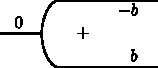
\includegraphics{diagrams/eta.pdf}
\end{center}

Note that the connective is a {{+}}, hence only one of the branches
may be inhabited at any time. Thus the action of {{eta}} is to
transfer a backward flowing value on one wire to a forward flowing
value on the other wire.

{{eps}}

\begin{center}
  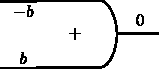
\includegraphics{diagrams/eps.pdf}
\end{center}

Coherence condition

\begin{center}
  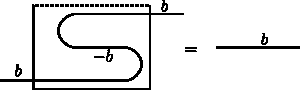
\includegraphics{diagrams/coherence.pdf}
\end{center}

Function

\begin{center}
  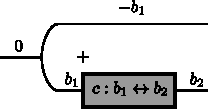
\includegraphics{diagrams/function.pdf}
\end{center}

Let us use the shorthand {{b1 -o b2 = -b1 + b2}}

Function application

\begin{center}
  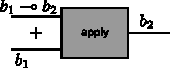
\includegraphics{diagrams/apply1.pdf}
\end{center}

\begin{center}
  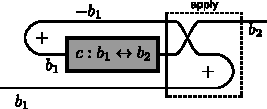
\includegraphics{diagrams/apply2.pdf}
\end{center}


Function composition

\begin{center}
  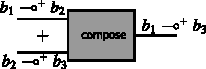
\includegraphics{diagrams/compose1.pdf}
\end{center}

\begin{center}
  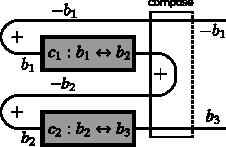
\includegraphics{diagrams/compose.pdf}
\end{center}

This is also equivalent to sequencing both the computation blocks. 

\begin{center}
  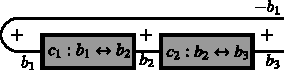
\includegraphics{diagrams/compose2.pdf}
\end{center}


Delimited continuation

\begin{center}
  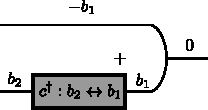
\includegraphics{diagrams/delimc.pdf}
\end{center}

Trace 

%subcode{proof} include main
%@ c : b2 + b1 <-> b2 + b3
%@@ trace c : b1 <-> b3

\begin{center}
  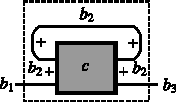
\includegraphics{diagrams/trace.pdf}
\end{center}

Double Negation

{{b <-> -(-b)}}

\begin{center}
  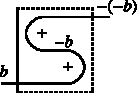
\includegraphics{diagrams/double_neg.pdf}
\end{center}

Negation distributes over {{+}}.

{{-(b1 + b2) <-> (b1) + (-b2)}}

\begin{center}
  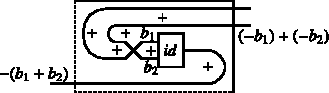
\includegraphics{diagrams/dist_neg_plus.pdf}
\end{center}

{{eps_{fst} }}

{{(-b1)*b2 + b1*b2 <-> 0}}

\begin{center}
  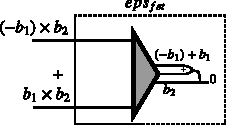
\includegraphics{diagrams/eps_fst.pdf}
\end{center}

Lifting negation out of {{*}}.

{{(-b1) * b2 <-> -(b1 * b2) <-> b1 * (-b2)}}

\begin{center}
  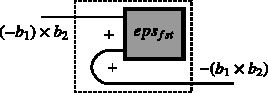
\includegraphics{diagrams/mult_neg.pdf}
\end{center}

The following isomoprhism can be constructed similarly 

{{b1 * b2 <-> (-b1)*(-b2)}}


Lifting a operation of postive types to negated types:

Given {{c : b1 <-> b2}}

\begin{center}
  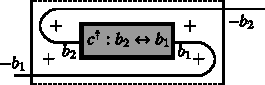
\includegraphics{diagrams/neg_lift.pdf}
\end{center}




\paragraph*{Observability.} 
Execution of program is defined by {{c : b1 <-> b2}} when evaluated on
input {{v1 : b1}} gives us a value {{v2 : b2}} on
termination. Execution is well defined only if {{b1}} and {{b2}} are
entirely positive types. Consider the program that

\begin{center}
  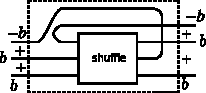
\includegraphics{diagrams/shuffle.pdf}
\end{center}

We define observables to be only positive types. The ouputs of
programs that ouput mixed positive and negative types are not
observable.  Also, programs that input mixed positive and negatives
types are not executable.

\subsection{To think about}

\begin{itemize}

\item If we built an effect over {{langRevEE}}, say {{create}} and
  {{erase}}, are effects structured by an arrow or a monad now?

\item Which operations can be lifted to work on negative types?

\item Can the operational semantics for {{langRevEE}} be an
  interpreter that is implemented in {{langRevT}} (similar to how the
  the tree traversal interpreter was implemented). This would imply
  the existence of a more powerful construction than Int, wherein the
  products would also be preserved. This is possibly worth a paper in
  itself.

\item These functions aren't really values. There is no value one can
  produce that denotes a function. These functions are the ability to
  transform a value - the possibility of transforming a value.  In the
  product encoding of environments, there is no value one can assign
  to a variable such that it denotes a function.


Actually this is possible. Consider two functions {{f : b1 <-> b2}}
and {{g : b1 <-> b2}}. A value of type {{bool}} is sufficient to
discriminate them. Hence the {{boo}} is the first class representation
of the functions and can be thought of as the address of the function. 

\begin{center}
  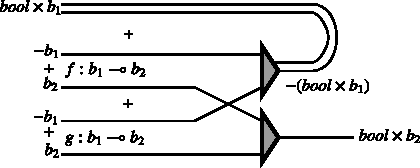
\includegraphics{diagrams/dispatch.pdf}
\end{center}


\item It is not fair to say that negative types flow backwards. The
  following circuits are valid in {{langRevEE}}. It is however proper
  to say that for any type {{b}} that flows in a direction, the type
  {{-b}} flows in the reverse direction. 

\begin{center}
  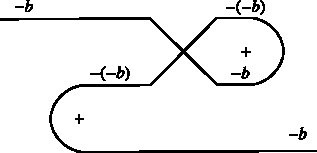
\includegraphics{diagrams/neg_circuit1.pdf}
\end{center}

\begin{center}
  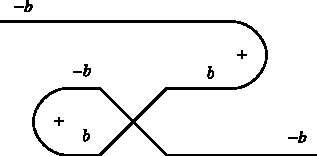
\includegraphics{diagrams/neg_circuit2.pdf}
\end{center}




\end{itemize}






%%%%%%%%%%%%%%%%%%%%%%%%%%%%%%%%%%%%%%%%%%%%%%%%%%%%%%%%%%%%%%%%%%%%%%%%%%%%%%%%
\section{Conclusion}

\acks This project was partially funded by Indiana University's Office
of the Vice President for Research and the Office of the Vice Provost
for Research through its Faculty Research Support Program.  We also
acknowledge support from Indiana University's Institute for Advanced
Study.

%%%%%%%%%%%%%%%%%%%%%%%%%%%%%%%%%%%%%%%%%%%%%%%%%%%%%%%%%%%%%%%%%%%%%%%%
\begin{small}
\bibliographystyle{abbrvnat}
\bibliography{cites}
\end{small}

\end{document}

%%%%%%%%%%%%%%%%%%%%%%%%%%%%%%%%%%%%%%%%%%%%%%%%%%%%%%%%%%%%%%%%%%%%%%%%
